\chapter{Evaluation}




\section{Implementation details}


Even though the authors of \cite{elden_savas_2007}
and \cite{IDLAVH09} provide the implementation 
of their methods in form of Matlab code,
it was necessary to reimplement this for two reasons.
First, we solve the Tucker2 decomposition problem, not the
full decomposition. It is not possible to use the existing 
code just supplying the same number for $I_1$
and $d_1$, because these methods use HOSVD as initialization step
and our tensors have dimension $17,988 \times 90 \times 25$.
Whereas we want the first factor matrix to be identity of the size
$17,988 \times 17,988$, the unfolding $X_{(1)}$ has the size
$17,988 \times 2,250$ and has at most $2,250$ 
non-zero singular values, so HOSVD will fail.
Second, and more important reason is that the implementation
provided by the authors is usually aimed at working
with relatively small tensors. In the intermediate calculations
it is necessary to compute the matrices whose
dimension for our data would be too big to fit into memory.
We overcome this issue by computing the matrix of the 
system column-wise. In \cite{IDLAVH09} the authors
used the GMRES solver to solve the system \ref{?} without
explicit computation of the matrix. This approach could
be adapted in our case, but it may be interesting
to look at the condition numbers of system matrices, 
so we decided to compute them explicitly.
Third, if some of this methods proved to be much more
efficient than HOOI, it would be necessary to integrate 
them into existing framework written in C++.

We  implemented the numerical methods in C++ using the existing framework 
of Bolkart and Wuhrer (\cite{bolkart_wuhrer_2013}).
The implementation was done with Armadillo library.
The differential-geometric Newton method was implemented in Matlab. 
We used tensor toolbox for this.
The code for fitting was provided as part of the framework. The code for 
expression recognition was taken from Daniel Mohr's thesis
(it had to be changed to work with full scans instead of their subset
that corresponds to Kinect landmarks).



\section{Protocol}

All experiments were conducted on the BU-3DFE database. The database contains $2,500$ scans of faces. There are $100$
persons ($50$ men and $50$ women) and each person performs $25$ expressions.
There is one neutral expression and every person expressed each of the $6$ emotions (anger, sadness,
happiness, surprise, disgust, fear) at $4$ intensity levels. The database is annotated, there are landmarks
with clear semantic meaning (like tip of the nose, eye corners, etc).
For training we need registered scans and we used the registration 
from \cite{Salazar}. It was performed with template fitting method
and some obvious mistakes were manually corrected by T. Bolkart.
The registered scans contain $5,996$ points each, so the mode-$1$ dimension
of the  uncompressed tensors is $17,988$.

We used the {$10$-fold} cross validation. 
The database was split into $10$ parts, each part containing the same number of males and females, and
each part was used as a testing dataset for models trained on the other $9$ parts, then the results
were averaged.

\section{Frobenius norm}

The simplest measure of comparing different methods
is calculating the Frobenius norm of the residual $|| X - M \times_2 F_2 \times_3 F_3 ||$.
The average values of Frobenius norm are given in {Table \ref{frob-norm-residual}}:


\begin{table}[h]
\centering
\begin{tabular}{|l|l|l|l|}
\hline
HOSVD & HOOI & NG & DGN \\ \hline
$11,756.3$  & $11,475.02$  & $11,475.0$ & $11,475.0$ \\ \hline
\end{tabular}
\caption{Values of the Frobenius norm of the residual. NG stands for Newton-Grassmann method, DGN stands for Differential-Geometric Newton Method.}
\label{frob-norm-residual}
\end{table}


We see that HOOI gives some improvement in comparison to HOSVD,
while the effect of Newton's methods is hardly noticeable (see remarks below). Note that it is the result of the
first $4$ iterations. In {Table \ref{hooi-improv}} we provide a typical dynamics of improvement
for HOOI. We can see that  after first $4$ or $5$ iterations the norm practically 
does not decrease and it makes no sense to run the process further.


We need to  make additional remarks about Newton's methods.
In out implementation of Newton-Grassmann and differential-geometric Newton
methods we had to change the update step. In the papers \cite{elden_savas_2007},
\cite{IDLAVH09} the step size is fixed to be $1$ (see formulas ...).
If we implement the methods this way, they diverge rapidly. In order to overcome
this we perform a simple search for a smaller step size that makes the objective
function smaller.
Notice that it is a general recommendation to use some optimization
for step size at each iteration in Newton's methods (\cite{num_recipes}).
We also had to apply the Gram-Schmidt 
orthogonalization process in the differential-geometric Newton method.


However, this behaviour is  not too surprising. One of the disadvantages
of Newton's methods is that they can diverge, if the initial value
is too far from the real root. It seems that in case of 
a large tensor we need to be closer to the optimum than HOOI (which we used
as initialization) can bring us to. As for Gram-Schmidt process,
the authors of \cite{IDLAVH09} did not claim that it is proven
that the process automatically converges to matrices with orthonormal 
columns. This was an empiric observation based on the experiments
with $10 \times 10 \times 10$ tensors. It might be that this statement
is  nevertheless true and we would not need this orthogonalization, if 
our initialization was better.



Comparing running time.

\begin{table}[h]
\centering
\begin{tabular}{|l|l|l|l|}
\hline
HOSVD & HOOI & NG & DGN \\ \hline
$30$  & $35$  & $120$ & $3,600$ \\ \hline
\end{tabular}
\caption{Values of the Frobenius norm of the residual}
\label{running_time_per_iteration}
\end{table}


We can also visualize this approximation error at each pixel:

\begin{figure}
        \centering
        \begin{subfigure}[b]{0.6\textwidth}
                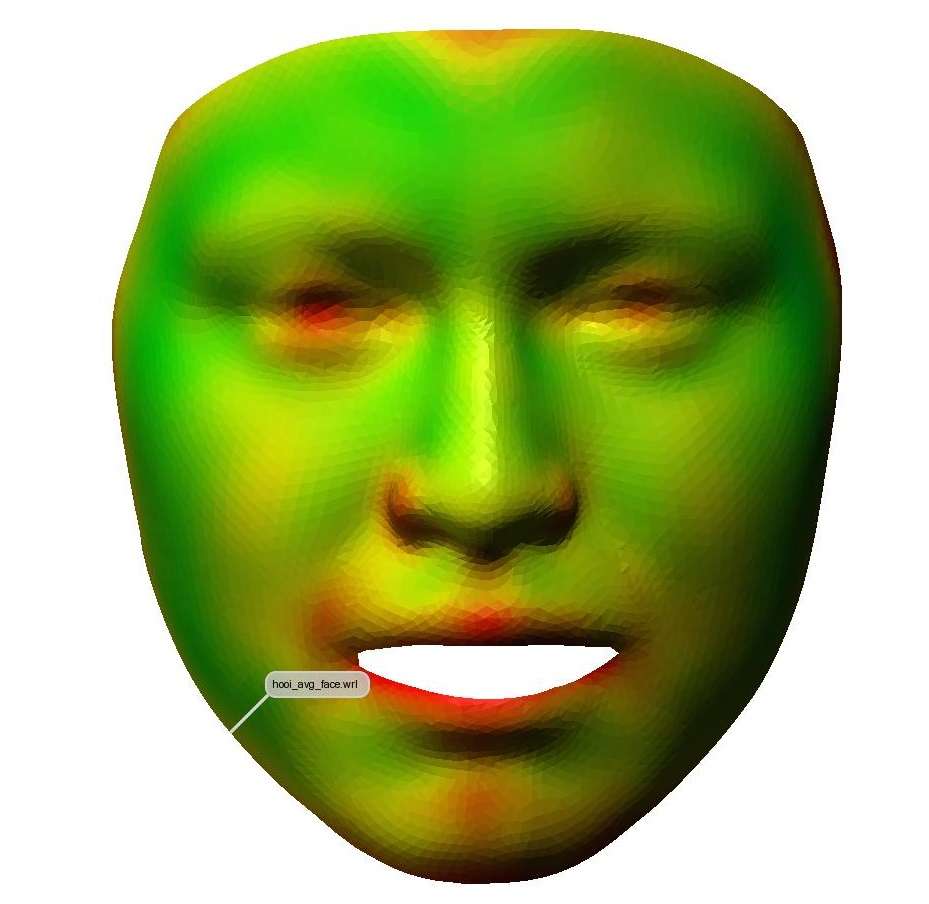
\includegraphics[width=\textwidth]{images/hooi_avg_face.jpg}
                \caption{HOOI}
                \label{HOOI_face}
        \end{subfigure}%
        ~ %add desired spacing between images, e. g. ~, \quad, \qquad etc.
          %(or a blank line to force the subfigure onto a new line)
        \begin{subfigure}[b]{0.55\textwidth}
                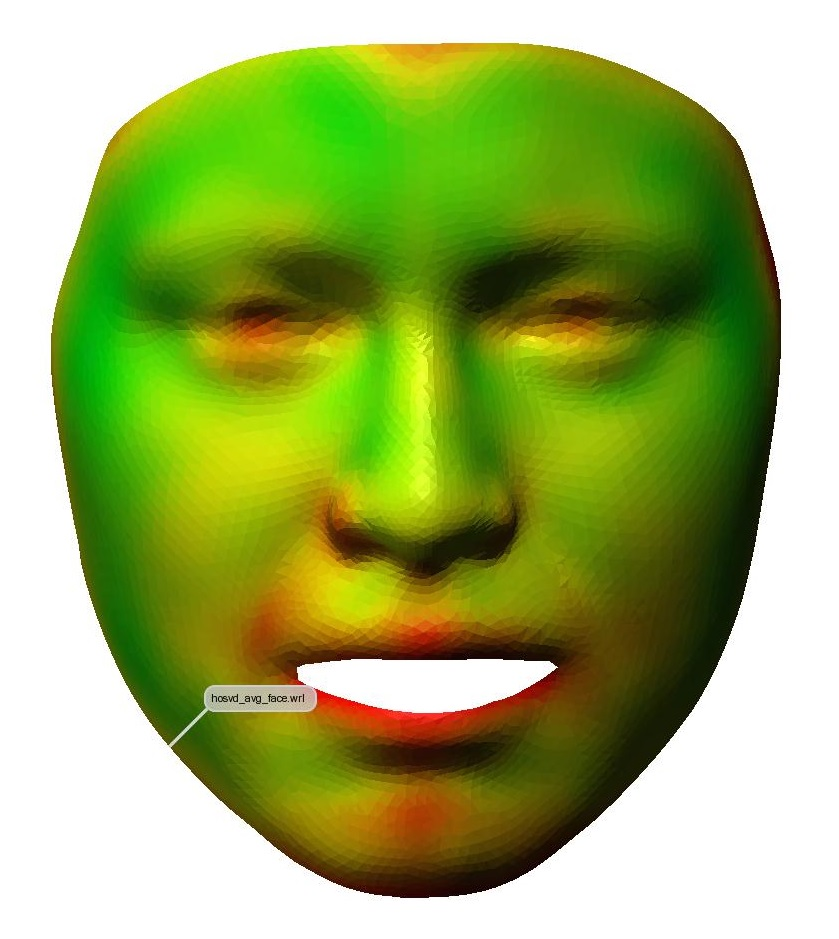
\includegraphics[width=\textwidth]{images/hosvd_avg_face.jpg}
                \caption{HOSVD}
                \label{HOSVD_face}
        \end{subfigure}
        \caption{Average error per point for HOOI and HOSVD models}
        \label{fig:hooi_hosvd_comparison}
\end{figure}

We see that HOOI gives some improvement 
, but the difference is not that big. On the other hand, if we compare the 
gradients of the cost function, we see that the result of HOOI is much closer to the 
critical point:

\begin{figure}
        \centering
                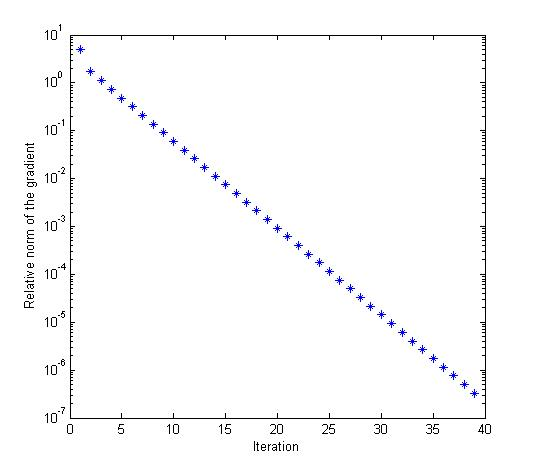
\includegraphics[width=8cm]{images/hooi_gradient_plot.jpg}
        \caption{Relative norm of the gradient (logarithmic scale).}
        \label{fig:hooi_grad_plot}
\end{figure}



\begin{figure}
        \centering
                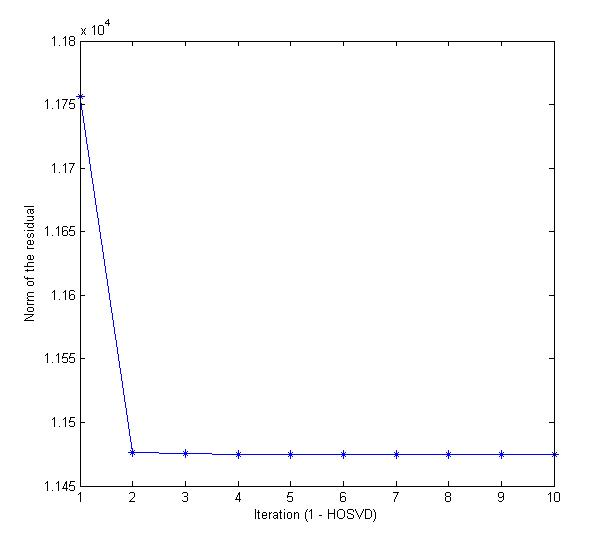
\includegraphics[width=8cm]{images/hooi_hosvd_residual_plot.jpg}
        \caption{Norm of the residual for HOOI, starting with HOSVD.}
        \label{fig:hooi_hosvd_resid_plot}
\end{figure}




\begin{figure}
        \centering
                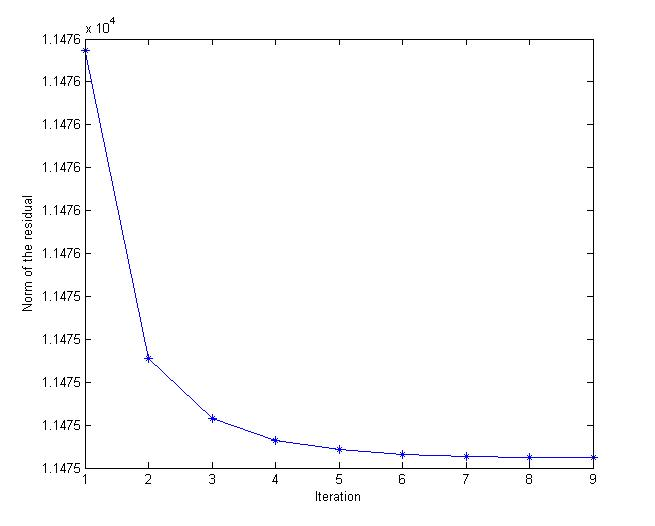
\includegraphics[width=8cm]{images/hooi_residual_plot.jpg}
        \caption{Norm of the residual for HOOI.}
        \label{fig:hooi_resid_plot}
\end{figure}

\section{Reconstruction and Fitting}
\label{eval_fit}
The more application-relevant measure is fitting error: we take face scans
from test dataset and try to fit them to the model. After that we measure the difference
between reconstructed face and the original scan (at points where we have found correspondence).
We can either use non-registered original data from testing dataset
or we can try to reconstruct the registered version of scans. The former case is 
standard fitting procedure, we refer to the latter case as reconstruction. The difference
between the two is in measuring errors: for fitting we simply use nearest neighbour,
e.g., for each point of the reconstructed face we find the nearest neighbour on the
original surface and sum up the distances between these pairs of points.
If we reconstruct registered data, we already have good correspondence
between points of the input scan and points on scans from the training dataset,
so we use this correspondence as groundtruth and sum up distances between 
points with the same index. This measure we call reconstruction error,
it is \textit{a priori} expected that it will be higher than the nearest neighbour
one, because we require more from our reconstruction.



\section{Expression Recognition}

The expression recognition test was performed using the method similar to that of Mpiperis et al (\cite{?}).
The first step is to train the multilinear model and then reconstruct
the scans from the training dataset using this model (that is, to compute 
$\X \times_2 F_2 \times_3 F_3$).  The input scan $\f$ from the testing dataset
is then registered using the multilinear model, too:
\begin{equation}
    f \approx \mu + X \times_2 w_2 \times_3 w_3 =: f_r.
\end{equation}



\begin{table}[h]
\centering
\begin{tabular}{|l|l|l|l|l|l|l|}
\hline
& Angry & Disgust & Fear & Happy & Sad & Surprised \\ \hline
Angry     & 210 &  70 &  14 &  4 &  102 &  0   \\ \hline
Disgust   & 76 &  264 &  22 &  15 &  15 &  8   \\  \hline
Fear      & 53 &  190 &  93 &  15 &  20 &  29   \\ \hline
Happy     & 15 &  186 &  112 &  81 &  3 &  3   \\  \hline
Sad       & 143 &  62 &  8 &  3 &  184 &  0   \\   \hline
Surprised & 83 &  124 &  27 &  1 &  52 &  113  \\ \hline
\end{tabular}
\caption{Confusion matrix for expression recognition, HOSVD }
\label{expr_rec_hosvd_confmatr}
\end{table}


\begin{table}[h]
\centering
\begin{tabular}{|l|l|l|l|l|l|l|}
\hline
& Angry & Disgust & Fear & Happy & Sad & Surprised \\ \hline
Angry     & 253 &  58 &  25 &  6 &  58 &  0   \\  \hline
Disgust   & 90 &  262 &  18 &  15 &  11 &  4   \\  \hline
Fear      & 64 &  178 &  99 &  19 &  13 &  27   \\ \hline
Happy     & 18 &  172 &  112 &  95 &  1 &  2   \\  \hline
Sad       & 199 &  43 &  9 &  1 &  146 &  2   \\   \hline
Surprised & 118 &  121 &  43 &  1 &  30 &  87  \\\hline
\end{tabular}
\caption{Confusion matrix for expression recognition, HOOI }
\label{expr_rec_hooi_confmatr}
\end{table}



\begin{table}[h]
\centering
\begin{tabular}{|l|l|l|l|l|l|l|}
\hline
& Angry & Disgust & Fear & Happy & Sad & Surprised \\ \hline
Angry     & 254 &  55 &  25 &  4 &  62 &  0 \\    \hline
Disgust   & 87 &  264 &  17 &  14 &  12 &  6 \\    \hline
Fear      & 69 &  174 &  100 &  19 &  11 &  27 \\ \\hline
Happy     & 18 &  170 &  115 &  94 &  1 &  2 \\    \hline
Sad       & 200 &  47 &  10 &  1 &  140 &  2 \\    \hline
Surprised & 119 &  121 &  42 &  0 &  32 &  86 \\  \hline
\end{tabular}
\caption{Confusion matrix for expression recognition, Newton-Grassmann}
\label{expr_rec_newgr_confmatr}
\end{table}


\begin{table}[h]
\centering
\begin{tabular}{|l|l|l|l|l|l|l|}
\hline
& Angry & Disgust & Fear & Happy & Sad & Surprised \\ \hline
Angry     & 254 &  54 &  23 &  5 &  64 &  0 \\  \hline
Disgust   & 83 &  268 &  15 &  15 &  11 &  8 \\  \hline
Fear      & 70 &  173 &  96 &  21 &  13 &  27 \\ \hline
Happy     & 19 &  169 &  117 &  91 &  1 &  3 \\  \hline
Sad       & 201 &  44 &  12 &  1 &  140 &  2 \\  \hline
Surprised & 118 &  116 &  45 &  1 &  35 &  85 \\ \hline
\end{tabular}
\caption{Confusion matrix for expression recognition, Differential-Geometric Newton}
\label{expr_rec_dg_newton_confmatr}
\end{table}

\begin{table}[h]
\centering
\begin{tabular}{|c|l|l|l|l|}
\hline
& HOSVD & HOOI & NG & DGN \\ \hline
Correctly classified & $945$  & $942$  & $938$ & $934$ \\ \hline
Classification rate& $39.37$  & $39.25$  & $39.08$ & $37.36$ \\ \hline
\end{tabular}
\caption{Expression recognition rate, comparison}
\label{expr_rec_rate_total}
\end{table}
